\color{black}
\section{Specifica componenti Romeo::View}
\label{specificaView}
\begin{figure} [!h]
\centering
	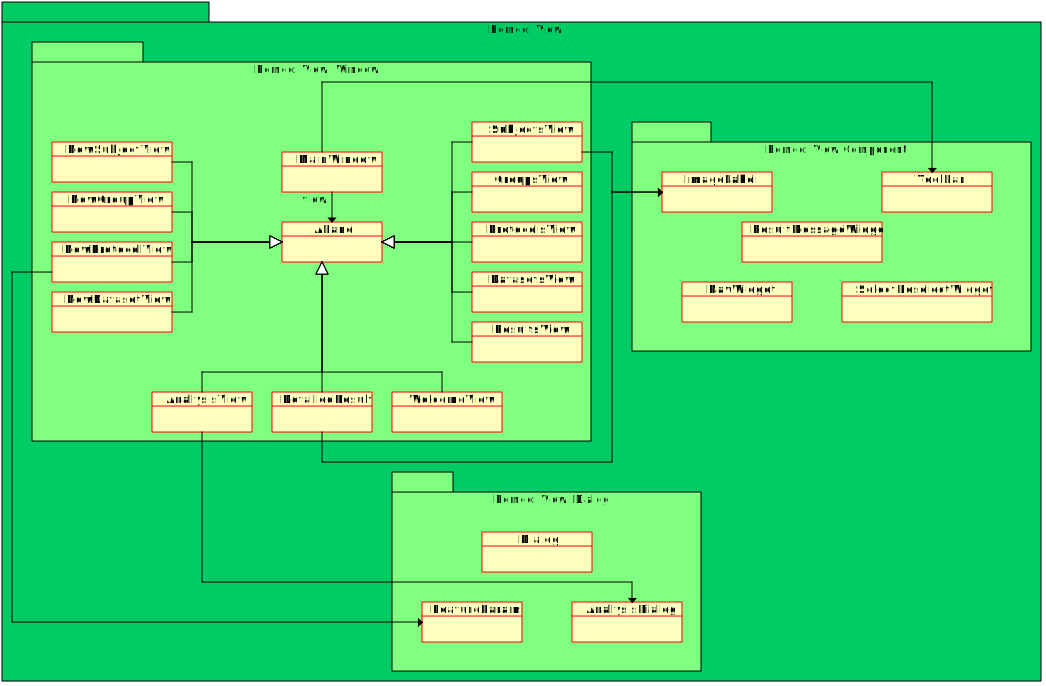
\includegraphics[width=0.8\linewidth] {../Specifica_Tecnica/Content/Immagini/RelazioniView.png}
			\caption{Componente Romeo::View}
			\label{comp_romeo::view}
\end{figure}
Package\g{} per il componente View dell'architettura MVC.
\subsection{Specifica componenti View::Window}
\label{specificaWindow}
\begin{figure}[!h]

			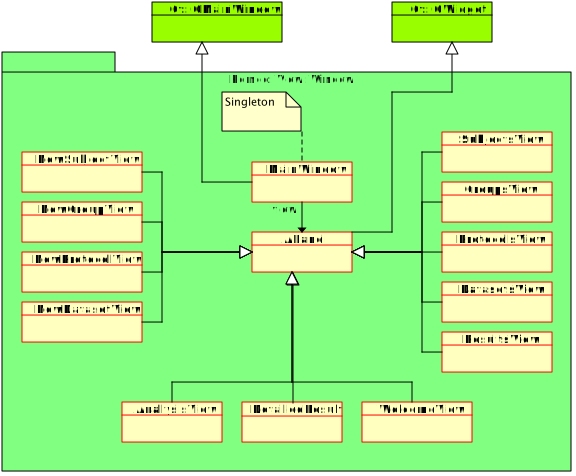
\includegraphics[width=0.8\linewidth]{../Specifica_Tecnica/Content/Immagini/Window.png}
			\caption{Componente Romeo::View::Window}
			\label{comp_romeo::view::window}
\end{figure}
Componente che contiene tutti i tipi di finestre disponibili nel sistema con cui l'utente potrà interagire per accedere alle funzionalità di \project.
\pagebreak
%%%%%%%%%%%%%%%%%%%%
%     MAINWINDOW
%%%%%%%%%%%%%%%%%%%%%%%
\subsubsection{MainWindow (class)}
\label{speMainWindow}
\begin{figure}[!h]
\centering
			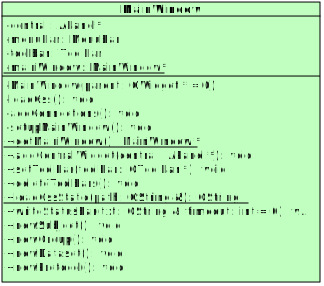
\includegraphics[width=0.6\linewidth]{./Content/Immagini/view/MainWindow.png}
			\caption{Diagramma Classe MainWindow: attributi e metodi}
			\label{cl_mainWind}
\end{figure}
\paragraph{Descrizione \\}
Classe che rappresenta la sola ed unica finestra attiva presente in \project{}. Dovendo essere l'unica istanza all'interno dell'applicativo, è stata implementata tramite design pattern\g{} Singleton.
\paragraph{Utilizzo\\}
La classe viene utilizzata per poter interagire con il core dell'applicazione mettendo a disposizione le varie funzionalità.
\paragraph{Classi ereditate\\}
\begin{itemize}
\item Qt::QMainWindow.
\end{itemize}
\paragraph{\color{black}Attributi \\}
\begin{itemize}
%APANEL
\item \color{teal}\verb!-  central: Window::APanel*!
\color{black}
\subparagraph{Descrizione:} Puntatore al widget che verrà impostato come centralWidget di MainWindow.

%MENUBAR
\item \color{teal}\verb!- shortcuts : QVector<QShortCut*>!
\color{black}
\subparagraph{Descrizione:} contiene la lista di shortcut disponibili per \project{}.
%TOOLBAR
\item \color{teal}\verb!-  toolBar : Component::ToolBar*!
\color{black}
\subparagraph{Descrizione:} Puntatore alla barra che darà la possibilità all'utente di filtrare e ordinare i dati. 

\item \color{teal}\verb!- static  mainWindow MainWindow*!
\color{black} 
\subparagraph{Descrizione:} Puntatore al campo dati statico che rappresenta l'unica istanza presente per la classe stessa, MainWindow che verrà istanziata in modo \emph{lazy} quando verrà richiesta la creazione dell'oggetto. 
\end{itemize}
%%%%%%%%%%%%% metodi %%%%%%%%%%%%%%%%5
\paragraph{\textcolor{black}{Metodi\\}}
\begin{itemize}
%costruttore
\item \color{blue}\verb!- MainWindow(parent : QWidget*=0)!
\color{black}
\subparagraph{Descrizione: }Costruttore privato (come prevede il design pattern\g{} Singleton) per la classe MainWindow. \\
\subparagraph{Argomenti}
\begin{itemize}
\item \color{RoyalPurple} \verb! parent : QWidget*=0 !\\ Puntatore al QWidget padre di MainWindow.
\end{itemize}
%LOADCSS
\item \color{blue}\verb!-loadCss():void!
\color{black} Metodo che carica il file contentente il css di default per MainWindow. \\
\subparagraph{Note}
 \begin{itemize}
 \item deve essere marcato costante.
 \end{itemize}

%SETUPMAINWINDOW
\item \color{blue}\verb!-setupMainWindow(): void !
\color{black}
\subparagraph{Descrizione:} Metodo che imposta la dimensione della finestra e la menuBar per la MainWindow.
 
%addConnections
\item \color{blue}\verb!-addConnections(): void!
\color{black} 
\subparagraph{Descrizione: }Metodo che si occupa di creare tutte le connessioni necessarie tra i vari oggetti che inviano un signal\g{} e quelli che implementano lo slot\g{} alla ricezione del signal\g{}.
 \subparagraph{Note:}
 \begin{itemize}
 \item deve essere marcato costante.
 \end{itemize}

%createShortcut
\item \color{blue}\verb!-createShortCuts(): void!
\color{black} 
\subparagraph{Descrizione: }Metodo che si occupa di creare gli shortcut disponibili.

%getMainWindow
\item \color{blue}\verb!+ static getMainWindow():MainWindow* !
\color{black}
\subparagraph{Descrizione:} Metodo statico che ritorna il puntatore all'unica istanza della classe MainWindow. Se l'istanza non esiste ancora, essa verrà creata e poi verrà ritornata. \\
\subparagraph{Note}
\begin{itemize}
\item deve essere un metodo statico.
\end{itemize}

 
%addCentralWidget
\item \color{blue}\verb!+addCentralWidget(central : APanel*):void !
\color{black}
\subparagraph{Descrizione:} Metodo che imposta l'oggetto puntato da central come central widget di MainWindow; central deve puntare a un oggetto sottotipo di APanel. \\
\subparagraph{Argomenti}
\begin{itemize}
\item \color{RoyalPurple}\verb! central : APanel* !\\ rappresenta il widget da settare come centralWidget di MainWindow.
\end{itemize}

%getToolBar
\item \color{blue}\verb!+ getToolBar() : QToolBar* !
\color{black}
\subparagraph{Descrizione: }
Metodo che ritorna un puntatore alla toolBar.
\subparagraph{Note}
\begin{itemize}
\item il metodo deve essere marcato come costante.
\end{itemize}

%loadCssStatic
\item \color{blue}\verb!+ loadCssStatic(path : const QString&): QString!
\color{black}
\subparagraph{Descrizione: }
 Metodo che apre e legge il file, il cui nome è contenuto in path, che contiene le impostazioni stilistiche per l'applicativo \project{} e ritorna il contenuto del file \\ 
 \subparagraph{Note}
 \begin{itemize}
 \item deve essere marcato statico;
 \item deve essere marcato costante.
 \end{itemize}
\subparagraph{Argomenti:}
\begin{itemize}
\item \color{RoyalPurple} \verb! path : const QString\& !\\ Stringa contenente il path del file da aprire e leggere.
\end{itemize}

%getShortCuts()
\item \color{blue}\verb!+ getShortCuts() : QVector<QShortCut*> !
\color{black}
\subparagraph{Descrizione: }
Metodo che ritorna un vettore contenente tutti gli shorcut per l'applicativo \project{}.
\subparagraph{Note:}
\begin{itemize}
\item il metodo deve essere marcato costante;
\end{itemize}

%setShortCutHomeEnable()
\item \color{blue}\verb!+ setShortcutHomeEnable(enable: bool) : void !
\color{black}
\subparagraph{Descrizione: }
Metodo che ha il compito di impostare lo shortcut per la pagina iniziale al valore definito dal parametro.
\subparagraph{Argomenti:}
\begin{itemize}
\item \color{RoyalPurple} \verb! enable: bool! \\ rappresenta il valore a cui deve essere impostata la proprietà dello shortcut per la pagina iniziale: true se è abilitato, false altrimenti.
\end{itemize}
\color{black}

%getCentralW()
\item \color{blue}\verb!+ getCentralWidget() : APanel* !
\color{black}
\subparagraph{Descrizione: }
Metodo che ritorna il puntatore al widget centrale della finestra principale.
\subparagraph{Note:}
\begin{itemize}
\item il metodo deve essere marcato costante;
\end{itemize}

%showHel()
\item \color{blue}\verb!+ showHelp(page: const QString\&) : void !
\color{black}
\subparagraph{Descrizione: }
Metodo che ha il compito di visualizzare la guida interattiva sull'utilizzo dell'applicativo \project{}.
\subparagraph{Argomenti:}
\begin{itemize}
\item \color{RoyalPurple} \verb! page: const QString\& !\\ Rappresenta la pagina dove la guida è chiamata.
\end{itemize}
\subparagraph{Note:}
\begin{itemize}
\item il metodo deve essere marcato costante;
\end{itemize}

%%%%%%% signals
\item \color{blue}\verb! + homeSC():void! (signal)
\color{black} 
\subparagraph{Descrizione:} Signal\g{} emesso quando lo shortcut \textit{home} è attivato.

\item \color{blue}\verb! + aboutSC():void! (signal)
\color{black} 
\subparagraph{Descrizione:} Signal\g{} emesso quando lo shortcut \textit{about} è attivato.

\item \color{blue}\verb! + exitSC():void! (signal)
\color{black} 
\subparagraph{Descrizione:} Signal\g{} emesso quando lo shortcut \textit{exit} è attivato.

\item \color{blue}\verb! + createNewSubjectSC():void! (signal)
\color{black} 
\subparagraph{Descrizione:} Signal\g{} emesso quando lo shortcut \textit{create new Subject} è attivato.

\item \color{blue}\verb! + createNewGroupSC():void! (signal)
\color{black} 
\subparagraph{Descrizione:} Signal\g{} emesso quando lo shortcut \textit{create new Group} è attivato.

\item \color{blue}\verb! + createNewProtocolSC():void! (signal)
\color{black} 
\subparagraph{Descrizione:} Signal\g{} emesso quando lo shortcut \textit{create new Protocol} è attivato.

\item \color{blue}\verb! + createNewDatasetSC():void! (signal)
\color{black} 
\subparagraph{Descrizione:} Signal\g{} emesso quando lo shortcut \textit{create new Dataset} è attivato.

\item \color{blue}\verb! + showSubjectsSC():void! (signal)
\color{black} 
\subparagraph{Descrizione:} Signal\g{} emesso quando lo shortcut \textit{manage Subjects} è attivato.

\item \color{blue}\verb! + showGroupsSC():void! (signal)
\color{black} 
\subparagraph{Descrizione:} Signal\g{} emesso quando lo shortcut \textit{manage Groups} è attivato.

\item \color{blue}\verb! + showProtocolsSC():void! (signal)
\color{black} 
\subparagraph{Descrizione:} Signal\g{} emesso quando lo shortcut \textit{manage Protocols} è attivato.

\item \color{blue}\verb! + showDatasetsSC():void! (signal)
\color{black} 
\subparagraph{Descrizione:} Signal\g{} emesso quando lo shortcut \textit{manage Datasets} è attivato.


\item \color{blue}\verb! + showResultsSC():void! (signal)
\color{black} 
\subparagraph{Descrizione:} Signal\g{} emesso quando lo shortcut \textit{show Results} è attivato.

\item \color{blue}\verb! + StartAnalysisSC():void! (signal)
\color{black} 
\subparagraph{Descrizione:} Signal\g{} emesso quando lo shortcut \textit{start analysis} è attivato.

\item \color{blue}\verb! + helpVideoGuideSC():void! (signal)
\color{black} 
\subparagraph{Descrizione:} Signal\g{} emesso quando lo shortcut \textit{video guide} è attivato.

\item \color{blue}\verb! + helpManualSC():void! (signal)
\color{black} 
\subparagraph{Descrizione:} Signal\g{} emesso quando lo shortcut \textit{interactive guide} è attivato.

\item \color{blue}\verb! + shortCutsSC():void! (signal)
\color{black} 
\subparagraph{Descrizione:} Signal\g{} emesso quando lo shortcut \textit{show shortcats} è attivato.

\item \color{blue}\verb! + helpPageSC():void! (signal)
\color{black} 
\subparagraph{Descrizione:} Signal\g{} emesso viene premuto il pulsante per l'help.

%%%% slot
% writeStatusBar
\item \color{blue}\verb!+ writeStatusBar(txt : const QString\&, timeout:int=0):void! (slot)
\color{black}
\subparagraph{Descrizione:} Slot\g{} che ha il compito di visualizzare la barra di stato attivato alla ricezione di un signal\g{}.\\ 
\subparagraph{Argomenti:}
\begin{itemize}
\item \color{RoyalPurple} \verb! txt : const QString\& !\\ Stringa contenente il testo da visualizzare;
\item \color{RoyalPurple} \verb! timeout: int=0! \\ intero che rappresenta il tempo per il quale il messaggio (txt) debba essere visualizzato: di default 0.
\end{itemize}
\end{itemize}
\color{black}
\pagebreak
%%%%%%%%%%%%%%%%%%
% 	APANEL
%%%%%%%%%%%%%%%%%
\subsubsection{APanel (abstract)}
\label{speAPanel}
\begin{figure}[!h]
\centering
			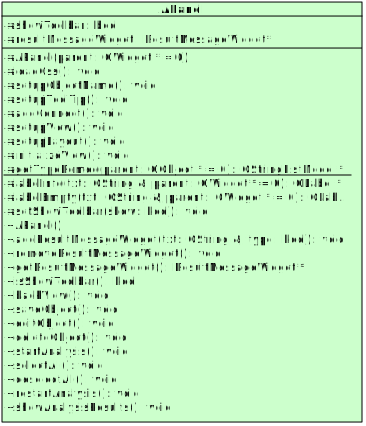
\includegraphics[width=0.65\linewidth]{./Content/Immagini/view/APanel.png}
			\caption{Diagramma Classe APanel: attributi e metodi}
			\label{cl_apanelV}
\end{figure}
\paragraph{Descrizione \\}
Classe che rappresenta il widget che verrà poi impostato come centralWidget di MainWindow.
\paragraph{Utilizzo\\}
La classe astratta fornisce dei contratti puri che verranno implementati dalle sottoclassi, e offre dei metodi disponibili alle sottoclassi.
\paragraph{Classi ereditate\\}
\begin{itemize}
\item Qt::QWidget.
\end{itemize}
%%%%%%%%%% attributi
\paragraph{\textcolor{black}{Attributi\\}}
\begin{itemize}
\item \color{teal}\verb!- showToolbar: bool!
\color{black}
\subparagraph{Descrizione: }Rappresenta un flag che vale true se la tool bar è visibile nella view, false atrimenti.
\item \color{teal} \verb! - resultMessageWidget: ResultMessageWidget*!
\subparagraph{Descrizione:} Puntatore alla componente che mostra all'utente il risultato dell'operazione eseguita sulla view (se è andata a buon fine o meno).
\end{itemize}

%%%%%%%%% metodi
\paragraph{\textcolor{black}{Metodi\\}}
\begin{itemize}
%costruttore
\item \color{blue}\verb! # APanel(parent : QWidget*=0)!
\color{black}
\subparagraph{Descrizione: }Costruttore protetto per la classe APanel.
\subparagraph{Argomenti}
\begin{itemize}
\item \color{RoyalPurple} \verb!parent : QWidget*=0! \\ Puntatore al QWidget padre di APanel.
\end{itemize}

%setupLayout
\item \color{blue}\verb! #setupLayout(): void !
\color{black}
\subparagraph{Descrizione:} Metodo virtuale puro che ha come contratto la costruzione del layout del widget. Il metodo deve essere ridefinito dalle classi che ereditano da questa, definendo la costruzione del proprio layout.
\subparagraph{Note:}
\begin{itemize}
\item questo metodo deve essere marcato virtuale puro;
\item questo metodo deve essere ridefinito.
\end{itemize}

%LOADCSS
\item \color{blue}\verb! #loadCss(): void !
\color{black} 
\subparagraph{Descrizione:} Metodo virtuale puro che ha come contratto il caricamento del file contentente il css per il widget. Il metodo deve essere ridefinito dalle classi che ereditano da questa, definendo il proprio css, qualora ne sia provvisto, altrimenti avrà corpo vuoto. \\ 
 \subparagraph{Note:}
 \begin{itemize}
 \item questo metodo deve essere marcato virtuale puro;
 \item questo metodo deve essere ridefinito.
 \end{itemize}

%setupObjectName
\item \color{blue}\verb! #setupObjectName():void!
\color{black}
\subparagraph{Descrizione:} Metodo virtuale puro con contratto quello di settare il nome ad ogni oggetto, contenuto nel widget. Il metodo deve essere ridefinito dalle classi che ereditano da questa, per gli oggetti contenuti nella classe. \\
 \subparagraph{Note:}
 \begin{itemize}
 \item questo metodo deve essere marcato virtuale puro;
 \item questo metodo deve essere ridefinito.
 \end{itemize}
  
%setupToolTip
\item \color{blue}\verb! #setupToolTip():void!
\color{black} 
\subparagraph{Descrizione: }Metodo virtuale puro che ha come contratto quello di settare i Tooltip\g{} agli oggetti della finestra. Il metodo deve essere ridefinito dalle classi che ereditano da questa impostando per ogni oggetto i ToolTip necessari per mostrare all'utente che sta utilizzando \project{} i suggerimenti e  spiegare a cosa serve quell'oggetto su cui si è posizionato con il cursore. \\
 \subparagraph{Note:}
 \begin{itemize}
 \item questo metodo deve essere marcato virtuale puro;
 \item questo metodo deve essere ridefinito.
 \end{itemize}
%addConnect
\item \color{blue}\verb! #addConnect(): void!
\color{black} 
\subparagraph{Descrizione:} Metodo virtuale puro che ha come contratto quello di fissare tutte le istruzioni \emph{connect}. Il metodo deve essere ridefinito dalle classi che ereditano da questa inserendo le connect necessarie al widget.\\ 
 \subparagraph{Note:}
 \begin{itemize}
 \item questo metodo deve essere marcato costante;
 \item questo metodo deve essere marcato virtuale puro;
 \item questo metodo deve essere ridefinito.
 \end{itemize}

%setupView
\item \color{blue}\verb! #setupView(): void !
\color{black} 
\subparagraph{Descrizione: } Metodo virtuale puro che ha come contratto quello di settare il layout del widget. Il metodo deve essere ridefinito dalle classi che ereditano da questa impostando il proprio layout.\\
 \subparagraph{Note:}
 \begin{itemize}
 \item questo metodo deve essere marcato virtuale puro;
 \item questo metodo è stato ridefinito.
 \end{itemize}
 

%initializeView
\item \color{blue}\verb! # initializeView(): void !
\color{black} 
\subparagraph{Descrizione: }
Metodo che invoca i metodi astratti precedentemente descritti, ridefiniti nella sottoclasse che eredita da APanel.

%getTypeRomeo
\item \color{blue}\verb! # static getTypeRomeo(parent:QObject*=0):QStringListModel*!
\color{black} 
\subparagraph{Descrizione:}
Metodo che ritorna una lista di stringhe usate dalla combobox per selezionare il tipo dell'immagine.
\subparagraph{Note:}
\begin{itemize}
\item il metodo deve essere marcato statico.
\end{itemize}
\color{black}

%labelInfo
\item \color{blue} \verb! # labelInfo(txt: const QString\&, parent:QWidget* =0): QLabel*! \\
\color{black}
\subparagraph{Descrizione:} Metodo che ha il compito di creare una label informativa da mostrare all'utente vicino ai campi di input; ritorna un puntatore alla label appena creata.
\subparagraph{Argomenti:}
\begin{itemize}
\item \color{RoyalPurple} \verb! txt: const QString\& ! \\Rappresenta il testo da mostrare all'utente;
\item \color{RoyalPurple} \verb! parent : QObject* ! \\ Puntatore al parent dell'oggetto label in creazione.
\end{itemize}
\subparagraph{Note:}
\begin{itemize}
\item il metodo deve essere marcato costante.
\end{itemize}

%labelEmpty
\item \color{blue} \verb! # labelEmpty(txt: const QString\&, parent:QWidget* =0): QLabel*! \\
\color{black}
\subparagraph{Descrizione:} Metodo che ha il compito di creare una label per mostrare all'utente una lista vuota; ritorna un puntatore alla label appena creata.
\subparagraph{Argomenti:}
\begin{itemize}
\item \color{RoyalPurple} \verb! txt: const QString\& ! \\Rappresenta il testo da mostrare all'utente;
\item \color{RoyalPurple} \verb! parent : QObject* ! \\ Puntatore al parent dell'oggetto label in creazione.
\end{itemize}
\subparagraph{Note:}
\begin{itemize}
\item il metodo deve essere marcato costante.
\end{itemize}

%setShowToolBar
\item \color{blue} \verb! # setShowToolBar(show : bool): void*! \\
\color{black}
\subparagraph{Descrizione:} Metodo che ha il compito di impostare se la toolbare è visibile o meno nella view in base al valore passato come parametro.
\subparagraph{Argomenti:}
\begin{itemize}
\item \color{RoyalPurple} \verb! show: bool! \\Rappresenta il valore a cui impostare il flag che dice se la toolbar è visibile (true) o meno.
\end{itemize}

%addResultMessag
\item \color{blue} \verb! + addResultMessageWidget(txt: const QString\&, type: bool):void! \\
\color{black}
\subparagraph{Descrizione:} Metodo che ha il compito di aggiungere il messaggio di risultato per avvenuta operazione o meno a seconda del valore del secondo parametro passato.
\subparagraph{Argomenti:}
\begin{itemize}
\item \color{RoyalPurple} \verb! txt: const QString\& ! \\Rappresenta il testo da mostrare all'utente all'interno del widget;
\item \color{RoyalPurple} \verb!type : bool ! \\ Vale true se il messaggio è un messaggio di successo, false se il messaggio è di errore.
\end{itemize}
\subparagraph{Note:}
\begin{itemize}
\item il metodo deve essere marcato virtuale.
\end{itemize}

%removeResultMessag
\item \color{blue} \verb! + removeResultMessageWidget():void! \\
\color{black}
\subparagraph{Descrizione:} Metodo che ha il compito di rimuovere il messaggio di risultato che l'utente sta visualizzando.

%isShowToolBar
\item \color{blue} \verb! + isShowToolbar():bool! \\
\color{black}
\subparagraph{Descrizione:} Metodo che il flag che dice se la toolbar è visibile o meno; ritorna true se la toolbar è visibile nella view, ritorna false se è nascosta.
\subparagraph{Note:}
\begin{itemize}
\item il metodo deve essere marcato costante.
\end{itemize}

%------------------------SIGNALS
%backview
\color{blue}\verb! + backView():void! (signal)
\color{black} 
\subparagraph{Descrizione: }
Signal\g{} emesso quando l'utente decide di ritornare alla vista precedente, ovvero quando viene premuto il pulsante back presente nelle viste che mettono a disposizione questa funzionalità.

%saveOb
\color{blue}\verb! + saveObject():void! (signal)
\color{black}
\subparagraph{Descrizione: }
Signal\g{} emesso quando l'utente decide di salvare le modifiche fatte nella vista corrente, ovvero quando viene premuto il pulsante save presente nelle viste che mettono a disposizione questa funzionalità.

%editObj
\color{blue}\verb! + editObject():void! (signal)
\color{black} 
\subparagraph{Descrizione: }
Signal\g{} emesso quando l'utente decide di modificare qualcosa nella vista corrente, ovvero quando viene premuto il pulsante edit presente nelle viste che mettono a disposizione questa funzionalità.

%deleteOb
\color{blue}\verb! + deleteObject():void! (signal)
\color{black} 
\subparagraph{Descrizione: }
Signal\g{} emesso quando l'utente decide di eliminare l'oggetto selezionato ovvero quando viene premuto il pulsante delete presente nelle viste che mettono a disposizione questa funzionalità.

%startAn
\color{blue}\verb! + startAnalysis():void! (signal)
\color{black} 
\subparagraph{Descrizione: }
Signal\g{} emesso quando l'utente decide avviare un'analisi, ovvero quando viene premuto il pulsante start Analysis presente nelle viste che mettono a disposizione questa funzionalità.

%selectAll
\color{blue}\verb! + selectAll():void! (signal)
\color{black} 
\subparagraph{Descrizione: }
Signal\g{} emesso quando l'utente decide selezionare tutti gil elementi presenti in una lista o tabella. Emesso dalle viste che mettono a disposizione questa funzionalità.

%deselectAll
\color{blue}\verb! + deselectAll():void! (signal)
\color{black} 
\subparagraph{Descrizione: }
Signal\g{} emesso quando l'utente decide deselezionare tutti gil elementi selezionati in una lista o tabella. Emesso dalle viste che mettono a disposizione questa funzionalità.

\item \color{blue}\verb! + restartAnalysis():void! (signal)
\color{black} 
\subparagraph{Descrizione: }
Signal\g{} emesso quando l'utente decide di far ripartire l'analisi, ovvero quando viene premuto il pulsante di restart analysis.

\item \color{blue}\verb! + showAnalysisResults():void! (signal)
\color{black} 
\subparagraph{Descrizione: }
Signal\g{} emesso quando l'utente decide di mostrare i risultati delle analisi, ovvero quando viene premuto il pulsante di visualizzazione dei risultati.
\end{itemize}
\pagebreak
%%%%%%%%%%%%%%%%%%%%%%%%%%%%%%%
%		WELCOMEVIEW
%%%%%%%%%%%%%%%%%%%%%%%%%%%%%%%
\subsubsection{WelcomeView (class)}
\label{speWelView}
\begin{figure}[!h]
\centering
			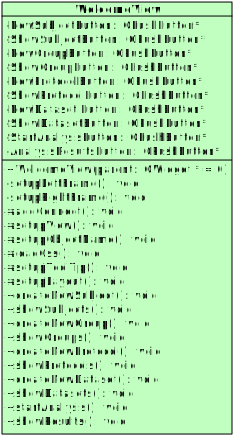
\includegraphics[width=0.4\linewidth]{./Content/Immagini/view/WelcomeView.png}
			\caption{Diagramma Classe WelcomeView: attributi e metodi}
			\label{cl_welcomeV}
\end{figure}
\paragraph{Descrizione \\}
Classe che rappresenta il widget della pagina iniziale, dove l'utente può scegliere le diverse operazioni da eseguire.
\paragraph{Utilizzo\\}
La classe implementerà i metodi virtuali puri della superclasse inoltre metterà a disposizione i pulsanti che daranno all'utente la possibilità di interagire con l'applicazione svolgendo l'operazione desiderata.
\paragraph{Classi ereditate\\}
\begin{itemize}
\item Window::APanel.
\end{itemize}
\paragraph{\textcolor{black}{Attributi\\}}
\begin{itemize}
%newSubjectButton
\item \color{teal}\verb!-newSubjectButton:QPushButton*!
\color{black}
\subparagraph{Descrizione: }pulsante per la creazione di un nuovo Subject\g{}. Alla pressione del pulsante verrà emesso un signal\g{} e verrà mostrata l'interfaccia per la creazione di un nuovo Subject\g{}.
 
%showSubjectButton
\item \color{teal}\verb!-showSubjectButton:QPushButton*!
\color{black}
\subparagraph{Descrizione: }pulsante per la visualizzazione dei Subject\g{} presenti nell'applicativo. Alla pressione del pulsante verrà emesso un signal\g{} e verrà mostrata l'interfaccia per la visualizzazione dei Subject\g{}.

%newGroupButton
\item\color{teal}\verb!-newGroupButton:QPushButton*!
\color{black}
\subparagraph{Descrizione: }pulsante per la creazione di un nuovo gruppo di Subject\g{}. Alla pressione del pulsante verrà emesso un signal\g{} e verrà mostrata l'interfaccia per la creazione di un nuovo gruppo di Subject\g{}.

%showGroupButton
\item\color{teal}\verb!-showGroupButton:QPushButton*!
\color{black}
\subparagraph{Descrizione: }pulsante per la visualizzazione dei gruppi di Subject\g{} presenti nell'applicativo e la possibilità di modificarne il contenuto, aggiungendo o togliendo Subject\g{} dal gruppo selezionato. Alla pressione del pulsante verrà emesso un signal\g{} e verrà mostrata l'interfaccia per la visualizzazione dei Subject\g{}.

%newProtocolButton
\item\color{teal}\verb!-newProtocolButton:QPushButton*!
\color{black}
\subparagraph{Descrizione: }pulsante per la creazione di un nuovo Protocol\g{}. Alla pressione del pulsante verrà emesso un signal\g{} e verrà mostrata l'interfaccia per la creazione di un nuovo Protocol\g{}.
 
%showProtocolButton
\item\color{teal}\verb!-showGroupButton:QPushButton*!
\color{black}
\subparagraph{Descrizione: }pulsante per la visualizzazione dei Protocol\g{} presenti nell'applicativo e la possibilità di eliminare quelli selezionati. Alla pressione del pulsante verrà emesso un signal\g{} e verrà mostrata l'interfaccia per la visualizzazione dei Subject\g{}.

%newDatasetButton
\item\color{teal}\verb!-newGroupButton:QPushButton*!
\color{black}
\subparagraph{Descrizione: }pulsante per la creazione di un nuovo Dataset\g{}. Alla pressione del pulsante verrà emesso un signal\g{} e verrà mostrata l'interfaccia per la creazione di un nuovo Dataset\g{}.

%showDatasetButton
\item\color{teal}\verb!-showDatasetButton:QPushButton*!
\color{black}
\subparagraph{Descrizione: }pulsante per la visualizzazione dei Dataset\g{} presenti nell'applicativo. Alla pressione del pulsante verrà emesso un signal\g{} e verrà mostrata l'interfaccia per la visualizzazione dei Dataset\g{}.

%startAnalysisButton
\item\color{teal}\verb!-showDatasetButton:QPushButton*!
\color{black}
\subparagraph{Descrizione: }pulsante per iniziare una nuova analisi. Alla pressione del pulsante verrà emesso un signal\g{} e verrà mostrata l'interfaccia per la creazione di una nuova analisi e la sua successiva esecuzione.

%analysisResultsButton
\item\color{teal}\verb!-analysisResultsButton:QPushButton*!
\color{black}
\subparagraph{Descrizione: }pulsante per la visualizzazione delle analisi effettuate con \project{} e i risultati prodotti da esse. Alla pressione del pulsante verrà emesso un signal\g{} e verrà mostrata l'interfaccia per la visualizzazione delle analisi presenti nell'applicativo.
\end{itemize}
\paragraph{\textcolor{black}{Metodi\\}}
\begin{itemize}
%%%%%%%%%%%%%%
%costruttore
\item\color{blue}\verb! + WelcomeView(parent : QWidget*=0)!
\color{black}
\subparagraph{Descrizione: }Costruttore per la classe WelcomeView. \\
\subparagraph{Argomenti:}
\begin{itemize}
\item \color{RoyalPurple} \verb! parent : QWidget*=0 !\\ Puntatore al QWidget padre di WelcomeView.
\end{itemize}

%%%%%%%%%%%%%%
%setupLeftFrame
\item\color{blue}\verb! - setupLeftFrame(): void!
\color{black}
\subparagraph{Descrizione: }Metodo che ha il compito di costruire la parte sinistra del widget iniziale.

%setupRightFrame
\item\color{blue}\verb! -setupRightFrame(): void !
\color{black}
\subparagraph{Descrizione: }Metodo che ha il compito di costruire la parte destra del widget iniziale.

%LOADCSS
\item\color{blue}\verb! #loadCss(): void !
\color{black} 
\subparagraph{Descrizione: }Metodo che implementa il contratto fornito dalla classe astratta \hyperref[speAPanel]{APanel}.\\
 \subparagraph{Note}
 \begin{itemize}
  \item questo metodo deve essere marcato virtuale;
 \item questo metodo è stato ridefinito.
 \end{itemize}

%setupObjectName
\item\color{blue}\verb! # setupObjectName():void!
\color{black}
\subparagraph{Descrizione: }
Metodo che implementa il contratto fornito dalla classe astratta \hyperref[speAPanel]{APanel}.\\
 \subparagraph{Note}
 \begin{itemize}
  \item questo metodo deve essere marcato virtuale;
 \item questo metodo è stato ridefinito.
 \end{itemize}
 
%setupToolTip
\item\color{blue}\verb! # setupToolTip(): void!
\color{black} 
\subparagraph{Descrizione: }Metodo che implementa il contratto fornito dalla classe astratta \hyperref[speAPanel]{APanel}.\\
 \subparagraph{Note}
 \begin{itemize}
 \item questo metodo deve essere marcato virtuale;
 \item questo metodo è stato ridefinito.
 \end{itemize}
 
%addConnect
\item\color{blue}\verb! #addConnect():void!
\color{black} 
\subparagraph{Descrizione: }Metodo che implementa il contratto fornito dalla classe astratta \hyperref[speAPanel]{APanel}.\\
 \subparagraph{Note}
 \begin{itemize}
 \item questo metodo deve essere marcato costante;
 \item questo metodo deve essere marcato virtuale;
 \item questo metodo è stato ridefinito.
 \end{itemize}

%setupView
\item\color{blue}\verb! #setupView():void!
\color{black}
\subparagraph{Descrizione: }
Metodo che implementa il contratto fornito dalla classe astratta \hyperref[speAPanel]{APanel}.
\subparagraph{Note:}
\begin{itemize}
\item questo metodo deve essere marcato virtuale;
\item questo metodo è stato ridefinito.
\end{itemize}
%%%%%%%%%%%%%%%%%% signal
\item\color{blue}\verb! + aboutus():void! (signal)
\color{black} 
\subparagraph{Descrizione:} Signal\g{} emesso quando viene premuto il pulsante \textit{about us}.

\item \color{blue}\verb! + exitSignal():void! (signal)
\color{black} 
\subparagraph{Descrizione:} Signal\g{} emesso quando viene premuto il pulsante \textit{exit}.

\item \color{blue}\verb! + createNewSubject():void! (signal)
\color{black} 
\subparagraph{Descrizione:} Signal\g{} emesso quando viene premuto il pulsante \textit{new Subject}.

\item \color{blue}\verb! + createNewGroup():void! (signal)
\color{black} 
\subparagraph{Descrizione:} Signal\g{} emesso quando viene premuto il pulsante \textit{new Gruop}.

\item \color{blue}\verb! + createNewProtocol():void! (signal)
\color{black} 
\subparagraph{Descrizione:} Signal\g{} emesso quando viene premuto il pulsante \textit{new  Protocol}.

\item \color{blue}\verb! + createNewDataset():void! (signal)
\color{black} 
\subparagraph{Descrizione:} Signal\g{} emesso quando viene premuto il pulsante \textit{new Dataset}.

\item \color{blue}\verb! + showSubjects():void! (signal)
\color{black} 
\subparagraph{Descrizione:} Signal\g{} emesso quando viene premuto il pulsante \textit{show Subjects}.

\item \color{blue}\verb! + showGroups():void! (signal)
\color{black} 
\subparagraph{Descrizione:} Signal\g{} emesso quando viene premuto il pulsante \textit{show Groups}.

\item \color{blue}\verb! + showProtocols():void! (signal)
\color{black} 
\subparagraph{Descrizione:} Signal\g{} emesso quando viene premuto il pulsante \textit{show Protocols}.

\item \color{blue}\verb! + showDatasets():void! (signal)
\color{black} 
\subparagraph{Descrizione:} Signal\g{} emesso quando viene premuto il pulsante \textit{show Dataset}.

\item \color{blue}\verb! + showResults():void! (signal)
\color{black} 
\subparagraph{Descrizione:} Signal\g{} emesso quando viene premuto il pulsante \textit{show Results}.

\item \color{blue}\verb! + StartAnalysis():void! (signal)
\color{black} 
\subparagraph{Descrizione:} Signal\g{} emesso quando viene premuto il pulsante \textit{start analysis}.

\item \color{blue}\verb! + VideoGuide():void! (signal)
\color{black} 
\subparagraph{Descrizione:} Signal\g{} emesso quando viene premuto il pulsante \textit{video guide}.

\item \color{blue}\verb! + userGuide():void! (signal)
\color{black} 
\subparagraph{Descrizione:} Signal\g{} emesso quando viene premuto il pulsante \textit{interactive guide}.

\item \color{blue}\verb! + shortcutsList():void! (signal)
\color{black} 
\subparagraph{Descrizione:} Signal\g{} emesso quando viene premuto il pulsante \textit{show shortcuts}.
\end{itemize}
\color{black}
\pagebreak

%%%%%%%%%%%%%%%%%%%%%%%%%%%%%%%%%%%%%%%%%%%
%		NEWSUBJECTVIEW
%%%%%%%%%%%%%%%%%%%%%%%%%%%%%%%%%%%%%%%%%%%
\subsubsection{NewSubjectView (class)}
\label{speNsubV}
\begin{figure}[!h]
\centering
			\includegraphics[width=0.7\linewidth]{./Content/Immagini/view/NewSubjectView.png}
			\caption{Diagramma Classe NewSubjectView: attributi e metodi}
			\label{cl_nsubview}
\end{figure}
\paragraph{Descrizione \\}
Classe che rappresenta il widget per la creazione di un nuovo \subject{}.
\paragraph{Utilizzo\\}
La classe implementerà i metodi virtuali puri della superclasse inoltre darà la possibilità all'utente di inserire il nome del \subject{}, selezionare il file corrispondente all'immagine da analizzare, opzionalmente potrà scegliere il file per la maschera e infine salvare le operazioni fatte, o ritornare alla finestra iniziale.
\paragraph{Classi ereditate\\}
\begin{itemize}
\item Window::APanel.
\end{itemize}
\paragraph{\textcolor{black}{Attributi\\}}
\begin{itemize}
\item \color{teal}\verb!-subjectName: QString!
\color{black}
\subparagraph{Descrizione: }Stringa che rappresenta il nome del \subject{}.

\color{teal}\verb!-subjectImage: QString!
\color{black}
\subparagraph{Descrizione: }Stringa che rappresenta il percorso dell'immagine da associare al \subject{}.

\color{teal}\verb!-subjectMask: QString !
\color{black}
\subparagraph{Descrizione: }Stringa che rappresenta il percorso della maschera da associare all'immagine del \subject{}.

%typeSelected
\color{teal}\verb! -typeSelected: QString!
\color{black} 
\subparagraph{Descrizione: }
Stringa che rappresenta il tipo di immagine associata al Subject\g{} in creazione.

%searchFileButton
\color{teal}\verb!-searchFileButton: QPushButton* !
\color{black}
\subparagraph{Descrizione: }pulsante che quando verrà premuto, emetterà un signal\g{} e verrà aperta una finestra di dialogo per navigare il file system e selezionare il file contenente l'immagine da caricare.

%searchMaskButton
\color{teal}\verb!-searchMaskButton: QPushButton* !
\color{black}
\subparagraph{Descrizione: }pulsante che quando verrà premuto, emetterà un signal\g{} e verrà aperta una finestra di dialogo per navigare il file system e selezionare il file contenente la maschera da caricare.

\color{teal}\verb! bottomWidget:NavWidget*!
\color{black} 
\subparagraph{Descrizione: }
Puntatore al widget che rappresenta la parte bassa della finestra contentente i pulsanti necessari al salvataggio all'annullamento delle operazioni e tornare indietro.
\end{itemize}
%%%% METODI 
\paragraph{\textcolor{black}{Metodi\\}}
\begin{itemize}
%costruttore
\item \color{blue}\verb! + NewSubjectView(parent : QWidget*=0)!
\color{black}
\subparagraph{Descrizione: }
Costruttore per la classe NewSubjectView.
\subparagraph{Argomenti:}
\begin{itemize}
\item \color{RoyalPurple}\verb!parent: QWidget*=0 ! \\ Puntatore al QWidget padre di NewSubjectView.
\end{itemize}

%setupLayout()
\item \color{blue}\verb! #setupLayout():void!
\color{black}
Metodo che implementa il contratto fornito dalla classe astratta \hyperref[speAPanel]{APanel}.\\
\subparagraph{Note: }
\begin{itemize}
\item questo metodo deve essere marcato virtuale;
\item questo metodo è stato ridefinito.
\end{itemize}

%Top
\item \color{blue}\verb! -createTop():void!
\color{black}
\subparagraph{Descrizione: }
Metodo che ha il compito di costruire la parte in alto del widget contenente la form per l'inserimento dei dati necessari per la creazione di un nuovo \subject{}.
 
%createButtom
\item \color{blue}\verb! -createButtom():void!
\color{black}
\subparagraph{Descrizione: }
Metodo che ha il compito di costruire la parte in basso del widget contenente il pulsante per ritornare alla pagine iniziale, il pulsante per il salvataggio e l'accesso alla guida.

%LOADCSS
\item \color{blue}\verb! #loadCss():void!
\color{black}
\subparagraph{Descrizione: }
 Metodo che implementa il contratto fornito dalla classe astratta \hyperref[speAPanel]{APanel}.\\
 \subparagraph{Note}
 \begin{itemize}
  \item questo metododeve essere marcato virtuale;
 \item questo metodo è stato ridefinito.
 \end{itemize}
 
%setupObjectName
\item \color{blue}\verb! #setupObjectName():void!
\color{black}
\subparagraph{Descrizione: }
Metodo che implementa il contratto fornito dalla classe astratta \hyperref[speAPanel]{APanel}.\\
 \subparagraph{Note}
 \begin{itemize}
  \item questo deve essere marcato virtuale;
 \item questo metodo è stato ridefinito.
 \end{itemize}

%setupToolTip
\item \color{blue}\verb! #setupToolTip():void!
\color{black}
\subparagraph{Descrizione: }
Metodo che implementa il contratto fornito dalla classe astratta \hyperref[speAPanel]{APanel}.\\
 \subparagraph{Note}
 \begin{itemize}
 \item questo metodo deve essere marcato virtuale;
 \item questo metodo è stato ridefinito.
 \end{itemize}

%addConnect
\item \color{blue}\verb! #addConnect():void!
\color{black}
\subparagraph{Descrizione: }
Metodo che implementa il contratto fornito dalla classe astratta \hyperref[speAPanel]{APanel}.\\
 \subparagraph{Note}
 \begin{itemize}
 \item questo metodo deve essere marcato costante;
 \item questo metodo deve essere marcato virtuale;
 \item questo metodo è stato ridefinito.
 \end{itemize}
 
%setupView
\item \color{blue}\verb! #setupView():void!
\color{black}
\subparagraph{Descrizione: }
Metodo che implementa il contratto fornito dalla classe astratta \hyperref[speAPanel]{APanel}.\\
 \subparagraph{Note}
 \begin{itemize}
 \item questo metodo deve essere marcato virtuale;
 \item questo metodo è stato ridefinito.
 \end{itemize}
 
%addResultMessag
\item \color{blue} \verb! + addResultMessageWidget(txt: const QString\&, type: bool):void!
\color{black}
\subparagraph{Descrizione:} Metodo che ha il compito di aggiungere il messaggio di risultato per avvenuta operazione o meno a seconda del valore del secondo parametro passato.
\subparagraph{Argomenti:}
\begin{itemize}
\item \color{RoyalPurple} \verb! txt: const QString\& ! \\Rappresenta il testo da mostrare all'utente all'interno del widget;
\item \color{RoyalPurple} \verb!type : bool ! \\ Vale true se il messaggio è un messaggio di successo, false se il messaggio è di errore.
\end{itemize}
\subparagraph{Note:}
\begin{itemize}
\item il metodo deve essere marcato virtuale.
\end{itemize}
 
%setSubjectName
\item \color{blue}\verb! +setSubjectName(name: QString\&):void!
\color{black}
\subparagraph{Descrizione: }
Metodo che modifica il nome associato al \subject{} da creare.
 \subparagraph{Argomenti:}
 \begin{itemize}
\item \color{RoyalPurple} \verb!name : const QString\& !\\ riferimento costante alla stringa contentente il nuovo nome per il \subject{}.
\end{itemize}
 \subparagraph{Note:}
 \begin{itemize}
 \item questo metodo verrà invocato dal controller che si occupa di questa vista.
 \end{itemize}
 
%setImagePath
\item \color{blue}\verb! + setImagePath(path: QString\&):void !
\color{black} 
\subparagraph{Descrizione: }Metodo che modifica il path dell'immagine associata al \subject{} da creare. \\
  \subparagraph{Argomenti:}
 \begin{itemize}
\item \color{RoyalPurple} \verb!path : const QString\& !\\ riferimento costante alla stringa contentente il nuovo path dell'immagine per il \subject{}.
\end{itemize} 
 \subparagraph{Note}
 \begin{itemize}
 \item questo metodo verrà invocato dal controller che si occupa di questa vista.
 \end{itemize}

%setMaskPath
\item \color{blue}\verb! +setMaskPath(path: QString\&): void !
\color{black}
\subparagraph{Descrizione: }Metodo che modifica il path della maschera associata al \subject{} da creare. \\
  \subparagraph{Argomenti:}
 \begin{itemize}
\item \color{RoyalPurple} \verb! path : const QString\& !\\ riferimento costante alla stringa contentente il nuovo path della maschera per il \subject{}.
\end{itemize}
 \subparagraph{Note}
 \begin{itemize}
 \item questo metodo verrà invocato dal controller che si occupa di questa vista.
 \end{itemize}

%setTypeSelection
\item \color{blue}\verb! +setTypeSelection(type: const QString\&):void! 
\color{black} 
\subparagraph{Descrizione: }Metodo che modifica il tipo dell'immagine associata al \subject{} in creazione. \\
  \subparagraph{Argomenti:}
 \begin{itemize}
\item \color{RoyalPurple} \verb!type : const QString\& !\\ riferimento costante alla stringa contentente il nuovo tipo dell'immagine associata al  \subject{}.
\end{itemize}
 \subparagraph{Note}
 \begin{itemize}
 \item questo metodo verrà invocato dal controller che si occupa di questa vista.
 \end{itemize}

%resetFields
\item \color{blue}\verb! + resetFields(): void!
\color{black}
\subparagraph{Descrizione: }Metodo che imposta ai valori di default tutti i campi della view.

%enableSearchFile
\item \color{blue}\verb! + enableSearchFile(): void!
\color{black}
\subparagraph{Descrizione: }Metodo che imposta ad abilitata la ricerca nel fileSystem.

%disableSearchFile
\item \color{blue}\verb! + disableSearchFile(): void!
\color{black}
\subparagraph{Descrizione: }Metodo che imposta ad disabilitata la ricerca nel fileSystem.

%getSubjectName
\item \color{blue}\verb! + getSubjectName(): QString!
\color{black}
\subparagraph{Descrizione: }Metodo che restituisce un QString contenente il nome del \subject{}. 
 \subparagraph{Note: }
 \begin{itemize}
 \item questo metodo deve essere marcato costante.
 \end{itemize}

%getImagePath
\item \color{blue}\verb! + getImagePath(): QString!
\color{black}
\subparagraph{Descrizione: }Metodo che restituisce un QString contenente il path dell'immagine associata al \subject{}.
 \subparagraph{Note:}
 \begin{itemize}
 \item questo metodo deve essere marcato costante.
 \end{itemize}

%getMaskPath
\item \color{blue}\verb! + getMaskPath(): QString!
\color{black}
\subparagraph{Descrizione: }
 Metodo che restituisce un QString contenente il path della maschera associata al \subject{} \\
 \subparagraph{Note}
 \begin{itemize}
 \item questo metodo deve essere marcato costante.
 \end{itemize}

%getType sel
\item \color{blue}\verb! + getTypeSelected(): QString!
\color{black}
\subparagraph{Descrizione: }
 Metodo che restituisce un QString contenente il tipo selezionato.\\
 \subparagraph{Note}
 \begin{itemize}
 \item questo metodo deve essere marcato costante.
 \end{itemize}

%resetFields
\item \color{blue}\verb! + resetFields(): void!
\color{black}
\subparagraph{Descrizione: }
 Metodo che resetta la form, eliminando il contenuto di ogni campo mettendo le impostazioni di default.

%addimage
\item \color{blue}\verb! + addImage():void! (signal)
\color{black} 
\subparagraph{Descrizione: }
Signal\g{} emesso quando l'utente decide di cercare nel file system l'immagine da associare al \subject{} ovvero quando viene premuto il pulsante searchFileButton.

%addmask
\item \color{blue}\verb! + addMask():void! (signal)
\color{black} 
\subparagraph{Descrizione: }
Signal\g{} emesso quando l'utente decide di cercare nel file system la maschera da associare al \subject{} ovvero quando viene premuto il pulsante searchMaskButton.

%saveSub
\item \color{blue}\verb! + saveSubject():void! (signal)
\color{black} 
\subparagraph{Descrizione: }
Signal\g{} emesso quando l'utente decide di salvare il \subject{} appena creato, ovvero quando viene premuto il pulsante save contentuto in bottomWidget.

%nameTextch
\item \color{blue}\verb! + nameTextChanded(text:QString\&):void! (signal)
\color{black} 
\subparagraph{Descrizione: }
Signal\g{} emesso quando l'utente modifica il nome contenuto nella linea di testo per l'inseriemnto del nome del \subject.
\subparagraph{Argomenti:}
\begin{itemize}
\item \color{RoyalPurple} \verb!text: QString\& !\\ rappresenta il nuovo nome da assegnare al Subject\g{}. 
\end{itemize}

%imagegetextch
\item \color{blue}\verb! + imageTextChanded(text:QString\&):void! (signal)
\color{black} 
\subparagraph{Descrizione: }
Signal\g{} emesso quando l'utente modifica il file dell'immagine da associare al Subject\g{}.
\subparagraph{Argomenti:}
\begin{itemize}
\item \color{RoyalPurple} \verb!text: QString\& !\\ rappresenta il path della nuova immagine da associare al Subject\g{}. 
\end{itemize}

%maskchang
\item \color{blue}\verb! + maskTextChanded(text:QString\&):void! (signal)
\color{black} 
\subparagraph{Descrizione: }
Signal\g{} eemesso quando l'utente modifica il file dell'immagine da associare al Subject\g{}.
\subparagraph{Argomenti:}
\begin{itemize}
\item \color{RoyalPurple}\verb!text: QString\& !\\ rappresenta il path della nuova maschera da associare al Subject\g{}. 
\end{itemize}

\end{itemize}
\color{black}
\pagebreak
%
%%%%%%%%%%%%%%%%%%%%%%%%%%%%%%%%
%	NEWGROUPVIEW
%%%%%%%%%%%%%%%%%%%%%%%%%%%%%%%
\subsubsection{NewGroupView (class)}
\label{speNgroV}
\begin{figure}[!h]
\centering
			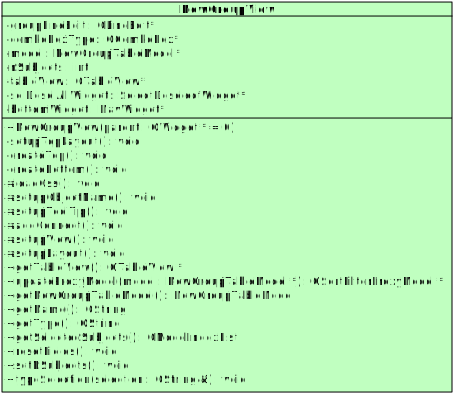
\includegraphics[width=0.75\linewidth]{./Content/Immagini/view/NewGroupView.png}
			\caption{Diagramma Classe NewGroupView: attributi e metodi}
			\label{cl_ngro}
\end{figure}
\paragraph{Descrizione \\}
Classe che rappresenta il widget per la creazione di un nuovo gruppo di \subject{}.
\paragraph{Utilizzo\\}
La classe implementerà i metodi virtuali puri della superclasse inoltre darà la possibilità all'utente di:
\begin{itemize}
\item inserire il nome del nuovo gruppo di \subject{};
\item selezionare il tipo dell'immagine che dovranno avere i \subject{} da aggiungere al gruppo;
\item selezionare, dalla lista dei \subject con associata un'immagine del tipo precedentemente scelto, i \subject{} di interesse;
\item salvare le operazioni fatte, o ritornare alla finestra iniziale.
\end{itemize}
\paragraph{Classi ereditate\\}
\begin{itemize}
\item Window::APanel.
\end{itemize}
\paragraph{\textcolor{black}{Attributi\\}}
\begin{itemize}
%model
\item \color{teal}\verb!-model: NewGroupTableModel* !
\color{black}
\subparagraph{Descrizione:}
Modello contenente i \subject{} contenuti nel gruppo 
%tableView
\item \color{teal}\verb!-tableView: QTabelView* !
\color{black}
\subparagraph{Descrizione:}
Contiene la lista dei \subject{} presenti in \emph{model}.

%nsub
\item\color{teal}\verb!-nSubject:int !
\color{black}
\subparagraph{Descrizione:}
Indica il numero di \subject{} presenti nel sistema con associata un'immagine del tipo indicato dal campo \emph{comboBoxType}.


%groupLine
\item \color{teal}\verb!-groupLineEdit: QLineEdit* !
\color{black}
\subparagraph{Descrizione:}
Linea di testo, contenente il nome del gruppo in creazione.

%comboBox
\item \color{teal}\verb!-comboBoxType: QComboBox* !
\color{black}
\subparagraph{Descrizione:}
Contiene l'elenco dei tipi di immagine che \project è in grado di elaborare; serve per selezionare poi i \subject{} che hanno il tipo di immagine indicato da questo campo dati.
\end{itemize}
%%%%%%%%%%%%%%%% metodi %%%%%%%%%%%%%%%%%%
\paragraph{\textcolor{black}{Metodi\\}}
\begin{itemize}
%costruttore
\item \color{blue}\verb! + NewGroupView(parent : QWidget*=0)!
\color{black}
\subparagraph{Descrizione:}
Costruttore per la classe NewGroupView. \\
\subparagraph{Argomenti}
\begin{itemize}
\item \color{RoyalPurple} \verb! parent: QWidget*=0 !\\ Puntatore al QWidget padre di NewGrouView.
\end{itemize}

%setupTopLayout
\item \color{blue}\verb! -setupTopLayout():void!
\color{black} 
\subparagraph{Descrizione:}
Metodo che ha il compito di impostare il layout in alto del widget, aggiungendo gli oggetti che lo compongono, e dando delle impostazioni grafiche.

%createTop
\item \color{blue}\verb! -createTop():void!
\color{black}
\subparagraph{Descrizione:} Metodo che ha il compito di costruire la parte in alto del widget contenente la form per l'inserimento dei dati necessari per la creazione di un nuovo gruppo di \subject{}.

%createButtom
\item \color{blue}\verb! -createButtom():void!
\color{black}
\subparagraph{Descrizione:}Metodo che ha il compito di costruire la parte in basso del widget contenente il pulsante per ritornare alla pagina iniziale, il pulsante per il salvataggio e l'accesso alla guida.

%setupLayout()
\item \color{blue}\verb! #setupLayout():void!
\color{black}
\subparagraph{Descrizione:}
Metodo che implementa il contratto fornito dalla classe astratta \hyperref[speAPanel]{APanel}.
\subparagraph{Note:}
\begin{itemize}
\item questo metodo deve essere marcato virtuale;
\item questo metodo è stato ridefinito.
\end{itemize}
 
%LOADCSS
\item \color{blue}\verb! #loadCss():void!
\color{black}
\subparagraph{Descrizione:}
Metodo che implementa il contratto fornito dalla classe astratta \hyperref[speAPanel]{APanel}.\\
 \subparagraph{Note}
 \begin{itemize}
  \item questo metodo deve essere marcato virtuale;
 \item questo metodo è stato ridefinito.
 \end{itemize}

%setupObjectName
\item \color{blue}\verb! #setupObjectName():void!
\color{black}
\subparagraph{Descrizione:}Metodo che implementa il contratto fornito dalla classe astratta \hyperref[speAPanel]{APanel}.\\
 \subparagraph{Note:}
 \begin{itemize}
  \item questo metodo deve essere marcato virtuale;
 \item questo metodo è stato ridefinito.
 \end{itemize}

%setupToolTip
\item \color{blue}\verb! #setupToolTip():void!
\color{black}
\subparagraph{Descrizione:}
Metodo che implementa il contratto fornito dalla classe astratta \hyperref[speAPanel]{APanel}.\\
 \subparagraph{Note}
 \begin{itemize}
 \item questo metodo deve essere marcato virtuale;
 \item questo metodo è stato ridefinito.
 \end{itemize}


%addResultMessag
\item \color{blue} \verb! + addResultMessageWidget(txt: const QString&, type: bool):void! \\
\color{black}
\subparagraph{Descrizione:} Metodo che ha il compito di aggiungere il messaggio di risultato per avvenuta operazione o meno a seconda del valore del secondo parametro passato.
\subparagraph{Argomenti:}
\begin{itemize}
\item \color{RoyalPurple} \verb! txt: const QString& ! \\Rappresenta il testo da mostrare all'utente all'interno del widget;
\item \color{RoyalPurple} \verb!type : bool ! \\ Vale true se il messaggio è un messaggio di successo, false se il messaggio è di errore.
\end{itemize}
\subparagraph{Note:}
\begin{itemize}
\item il metodo deve essere marcato virtuale.
\end{itemize}

%addConnect
\item \color{blue}\verb! #addConnect():void!
\color{black}
\subparagraph{Descrizione:} Metodo che implementa il contratto fornito dalla classe astratta \hyperref[speAPanel]{APanel}.
 \subparagraph{Note:}
 \begin{itemize}
 \item questo metodo deve essere marcato costante;
 \item questo metodo deve essere marcato virtuale;
 \item questo metodo è stato ridefinito.
 \end{itemize}
%setupView
\item \color{blue}\verb! #setupView():void!
\color{black}
\subparagraph{Descrizione:}
Metodo che implementa il contratto fornito dalla classe astratta \hyperref[speAPanel]{APanel}.\\
 \subparagraph{Note:}
 \begin{itemize}
 \item questo metodo deve essere marcato virtuale;
 \item questo metodo è stato ridefinito.
 \end{itemize}
%getTableView
\item \color{blue}\verb! + getTableView():QTableView*!
\color{black} 
\subparagraph{Descrizione:} Metodo che ritorna la tabella contenente tutti i \subject{} contenuti che gruppo.
%updateProxyMod
\item \color{blue}\verb! + updateProxyModel(): QSortFilterProxyModel*!
\color{black} 
\subparagraph{Descrizione:} Metodo che aggiorna il model della tabella dei \subject{} cliccando gli header della tabella stessa.
%getNewGroup
\item \color{blue}\verb! + getNewGroupTableModel(): NewGroupTableModel*!
\color{black} 
\subparagraph{Descrizione:}Metodo che ritorna il campo dati \emph{model}. 
\subparagraph{Note}
 \begin{itemize}
 \item questo metodo deve essere marcato costante.
 \end{itemize}
%getname
\item \color{blue}\verb! + getName(): QString!
\color{black} 
\subparagraph{Descrizione:}Metodo ch ritorna il nome del gruppo in creazione.
\subparagraph{Note:}
 \begin{itemize}
 \item questo metodo deve essere marcato costante.
 \end{itemize}
%getType
\item \color{blue}\verb! + getType(): QString!
\color{black} 
\subparagraph{Descrizione:}Metodo che ritorna il tipo di immagine che devono avere i \subject{} da inserire nel gruppo. 
\subparagraph{Note}
 \begin{itemize}
 \item questo metodo deve essere marcato costante.
 \end{itemize}

%getSelectedSubjects
\item \color{blue}\verb! + getSelectedSubjects(): QModelIndexList*!
\color{black} 
\subparagraph{Descrizione:}Metodo che ritorna la lista dei \subject selezionati.
\subparagraph{Note}
 \begin{itemize}
 \item questo metodo deve essere marcato costante.
 \end{itemize}

%resetForm
\item \color{blue}\verb! + resetFields(): void !
\color{black} 
\subparagraph{Descrizione:} Metodo che imposta tutti gli object contenuti dentro alla finestra al loro valore di default.

%setNsub
\item \color{blue}\verb! + setNSubjects(n: int):void!
\color{black} 
\subparagraph{Descrizione:} Metodo che imposta il campo dati \emph{nSubject}.
\subparagraph{Argomenti:}
 \begin{itemize}
 \item \color{RoyalPurple} \verb! n: int !\\numero di\subject{} presenti per il tipo selezionato, da assegnare al campo dati \emph{nSubject}.
 \end{itemize}
 
%setEditFields
\item \color{blue}\verb! + setEditFields (group: GroupsOfSubject*):void!
\color{black} 
\subparagraph{Descrizione:} Metodo che imposta i campi con i valori.
\subparagraph{Argomenti:}
 \begin{itemize}
 \item \color{RoyalPurple} \verb! group: GroupOfSubject* !\\ Rappresenta il puntatore al gruppo da editare.
 \end{itemize} 
 
%typeSelection
\item \color{blue}\verb! + typeSelection(selection: QString&):void! (signal)
\color{black}
\subparagraph{Descrizione:}
Signal\g{} emesso quando l'utente ha selezionato il tipo dalla combobox.
\subparagraph{Argomenti:}
\begin{itemize}
\item \color{RoyalPurple} \verb! selection: QString& ! \\ Rappresenta la stringa selezionata dall'utente.
\end{itemize}
\end{itemize}
\color{black}
\pagebreak


